\chapter{The Fisher Information Matrix}
\label{ch:fisher_info}

\section{The Geometry of Parameter Estimation}

In the paradigm of deep learning and statistical inference, we view learning as the act of selecting a single probability distribution from a parametrized family. When we train a neural network $f_\theta$ parameterized by $\theta \in \mathbb{R}^d$, we are navigating a high-dimensional manifold of probability distributions. Each distinct configuration of the weights $\theta$ instantiates a conditional distribution $p_\theta(y|x)$ (or an unconditional generative model $p_\theta(x)$), which maps inputs to predictions. However, the Euclidean geometry of the parameter space $\mathbb{R}^d$ is fundamentally misleading. A large Euclidean step in $\theta$-space might leave the output distribution almost completely unchanged, while a microscopic step in a different direction could catastrophically alter the network's predictions.

To understand learning mathematically, we must separate the parameters themselves from the statistical behavior they induce. The parameters $\theta$ are merely a coordinate system for a statistical manifold; they are an arbitrary choice of nomenclature for the underlying models. The true distance between two models must be measured in the space of distributions, relying on information-theoretic constructs such as the Kullback-Leibler divergence $D_{\text{KL}}$. When we examine the local geometry of this space---the infinitesimal neighborhoods around a specific model $p_\theta$---we arrive at the \textit{Fisher Information Matrix} (FIM).

The Fisher Information Matrix quantifies the amount of information that an observable random variable $X$ carries about an unknown parameter $\theta$ upon which the probability of $X$ depends. Intuitively, if the probability density function $p(x|\theta)$ is extremely sensitive to infinitesimal changes in $\theta$, then a sample from $X$ will provide a large amount of information regarding the true value of $\theta$. This sensitivity manifests geometrically as the curvature of the log-likelihood function. Where the log-likelihood is sharply peaked, the curvature is high, the Fisher Information is large, and the parameter can be estimated with high precision. Where the log-likelihood is flat, the Fisher Information is low, and the parameter is highly uncertain, yielding phenomena like the ``flat minima'' widely discussed in deep learning.

Furthermore, in the context of information geometry, the Fisher Information Matrix serves as the Riemannian metric tensor of the statistical manifold. It provides an intrinsic notion of distance, angle, and volume that is invariant to reparameterization. This foundational concept not only imposes absolute bounds on the variance of any unbiased estimator via the Cramér-Rao Lower Bound, but it also forms the basis for Natural Gradient Descent, a second-order optimization method that scales the parameter updates by the inverse of the FIM to achieve invariant convergence behavior.

In this chapter, we transition from the macroscopic quantities of information theory---entropy, mutual information, and divergence---to their differential and geometric counterparts. We will rigorously construct the Fisher Information Matrix, establish its equivalence to the expected Hessian of the log-likelihood, connect it directly to the Kullback-Leibler divergence, and demonstrate its application as a metric tensor. 

\section{The Score Function and Fisher Information}

We consider a parametrized family of probability distributions $p(x|\theta)$, where $x \in \mathcal{X}$ is a random variable and $\theta = [\theta_1, \dots, \theta_d]^T \in \Theta \subseteq \mathbb{R}^d$ is the parameter vector. We assume that $p(x|\theta)$ is strictly positive for all $x \in \mathcal{X}$ and $\theta \in \Theta$, and that the derivative with respect to $\theta$ exists and can be interchanged with the integral over $\mathcal{X}$ (regularity conditions).

\begin{definition}[Score Function]
The score function, or simply the score, is the gradient of the log-likelihood with respect to the parameter vector $\theta$:
\begin{equation}
    s(\theta; x) = \nabla_\theta \log p(x|\theta) = \begin{bmatrix}
        \frac{\partial}{\partial \theta_1} \log p(x|\theta) \\
        \vdots \\
        \frac{\partial}{\partial \theta_d} \log p(x|\theta)
    \end{bmatrix}
\end{equation}
\end{definition}

The score function indicates the direction and magnitude of the steepest ascent on the log-likelihood surface for a given observation $x$. Crucially, under the true distribution $p(x|\theta)$, the expected value of the score function is exactly zero.

\begin{theorem}[Zero Mean of the Score]
\label{thm:zero_mean_score}
Assuming that integration with respect to $x$ and differentiation with respect to $\theta$ commute, the expected value of the score function with respect to the distribution parameterized by $\theta$ is zero:
\begin{equation}
    \mathbb{E}_{x \sim p(x|\theta)}[s(\theta; x)] = \mathbf{0}
\end{equation}
\end{theorem}
\begin{proof}
We evaluate the expectation directly:
\begin{align*}
    \mathbb{E}_{x \sim p(x|\theta)}[\nabla_\theta \log p(x|\theta)] &= \int_{\mathcal{X}} p(x|\theta) \nabla_\theta \log p(x|\theta) \, dx \\
    &= \int_{\mathcal{X}} p(x|\theta) \frac{\nabla_\theta p(x|\theta)}{p(x|\theta)} \, dx \quad \text{(Chain Rule)} \\
    &= \int_{\mathcal{X}} \nabla_\theta p(x|\theta) \, dx \\
    &= \nabla_\theta \int_{\mathcal{X}} p(x|\theta) \, dx \quad \text{(Interchange integral and derivative)} \\
    &= \nabla_\theta (1) = \mathbf{0}
\end{align*}
\end{proof}

Because the expected score is zero, its covariance matrix is simply the expected outer product of the score with itself. This covariance matrix is defined as the Fisher Information Matrix.

\begin{definition}[Fisher Information Matrix]
The Fisher Information Matrix (FIM), denoted $F(\theta) \in \mathbb{R}^{d \times d}$, is the covariance matrix of the score function:
\begin{equation}
    F(\theta) = \mathbb{E}_{x \sim p(x|\theta)}\left[ s(\theta; x) s(\theta; x)^T \right] = \mathbb{E}_{x \sim p(x|\theta)}\left[ \nabla_\theta \log p(x|\theta) \nabla_\theta \log p(x|\theta)^T \right]
\end{equation}
\end{definition}

By definition, $F(\theta)$ is a symmetric and positive semi-definite matrix. If the parameters are identifiable (i.e., different $\theta$ map to different distributions), $F(\theta)$ is typically positive definite.

\subsection{Fisher Information as Expected Curvature}

While the FIM is defined via the first derivatives of the log-likelihood, it intimately relates to the second derivatives (the Hessian). This relationship provides the geometric intuition of Fisher Information as the expected curvature of the log-likelihood surface.

\begin{theorem}[FIM as Negative Expected Hessian]
\label{thm:fim_hessian}
Under the regularity conditions allowing the interchange of integration and double differentiation, the Fisher Information Matrix is equal to the negative expected Hessian of the log-likelihood:
\begin{equation}
    F(\theta) = - \mathbb{E}_{x \sim p(x|\theta)}\left[ \nabla_\theta^2 \log p(x|\theta) \right]
\end{equation}
\end{theorem}
\begin{proof}
Consider the Hessian of the log-likelihood. Applying the quotient rule to $\nabla_\theta \log p(x|\theta) = \frac{\nabla_\theta p(x|\theta)}{p(x|\theta)}$, we obtain:
\begin{align*}
    \nabla_\theta^2 \log p(x|\theta) &= \nabla_\theta \left( \frac{\nabla_\theta p(x|\theta)}{p(x|\theta)} \right) \\
    &= \frac{p(x|\theta) \nabla_\theta^2 p(x|\theta) - \nabla_\theta p(x|\theta) \nabla_\theta p(x|\theta)^T}{p(x|\theta)^2} \\
    &= \frac{\nabla_\theta^2 p(x|\theta)}{p(x|\theta)} - \left( \frac{\nabla_\theta p(x|\theta)}{p(x|\theta)} \right) \left( \frac{\nabla_\theta p(x|\theta)}{p(x|\theta)} \right)^T \\
    &= \frac{\nabla_\theta^2 p(x|\theta)}{p(x|\theta)} - s(\theta; x) s(\theta; x)^T
\end{align*}
Now, taking the expectation over $p(x|\theta)$:
\begin{align*}
    \mathbb{E}_{x \sim p(x|\theta)}\left[ \nabla_\theta^2 \log p(x|\theta) \right] &= \int_{\mathcal{X}} p(x|\theta) \frac{\nabla_\theta^2 p(x|\theta)}{p(x|\theta)} \, dx - \mathbb{E}_{x \sim p(x|\theta)}\left[ s(\theta; x) s(\theta; x)^T \right] \\
    &= \int_{\mathcal{X}} \nabla_\theta^2 p(x|\theta) \, dx - F(\theta) \\
    &= \nabla_\theta^2 \left( \int_{\mathcal{X}} p(x|\theta) \, dx \right) - F(\theta) \\
    &= \nabla_\theta^2 (1) - F(\theta) = -F(\theta)
\end{align*}
Multiplying by $-1$ completes the proof.
\end{proof}

This theorem is profoundly important for deep learning. The loss function $\mathcal{L}(\theta)$ is typically the expected negative log-likelihood over a dataset $\mathcal{D}$. The true Hessian of the expected loss is exactly the Fisher Information Matrix. Therefore, regions with high Fisher Information possess sharp minima, and regions with low Fisher Information correspond to flat minima.

\begin{figure}[htbp]
\centering
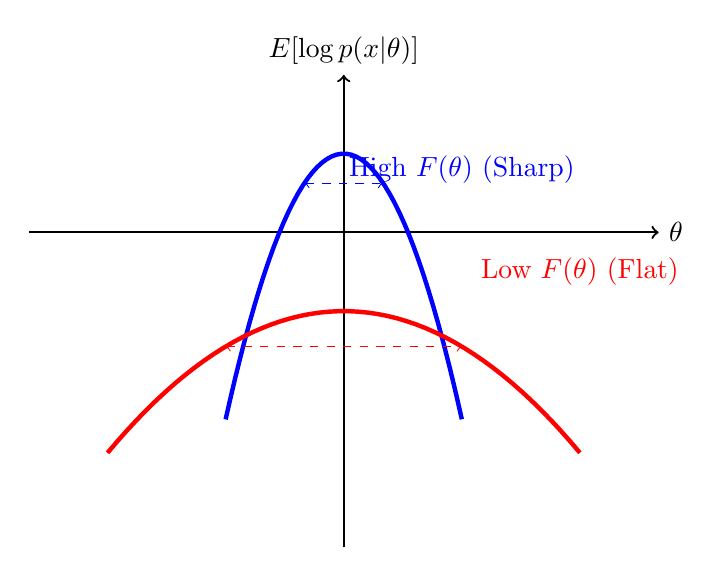
\begin{tikzpicture}
    % Axis
    \draw[->, thick] (-4,0) -- (4,0) node[right] {$\theta$};
    \draw[->, thick] (0,-4) -- (0,2) node[above] {$\mathbb{E}[\log p(x|\theta)]$};
    
    % High Fisher Information (sharp peak)
    \draw[ultra thick, blue, domain=-1.5:1.5, samples=50] plot (\x, {-1.5*\x*\x + 1});
    \node[blue] at (1.5, 0.8) {High $F(\theta)$ (Sharp)};
    
    % Low Fisher Information (flat peak)
    \draw[ultra thick, red, domain=-3:3, samples=50] plot (\x, {-0.2*\x*\x - 1});
    \node[red] at (3, -0.5) {Low $F(\theta)$ (Flat)};
    
    % Tangents/Curvature indicators
    \draw[<->, blue, dashed] (-0.5, 0.625) -- (0.5, 0.625);
    \draw[<->, red, dashed] (-1.5, -1.45) -- (1.5, -1.45);
\end{tikzpicture}
\caption{Geometric interpretation of the Fisher Information Matrix as curvature. The blue curve exhibits a sharp peak, corresponding to a highly negative expected Hessian (high Fisher Information). The red curve is relatively flat, indicating low curvature and low Fisher Information.}
\label{fig:fisher_curvature}
\end{figure}

\section{Connection to Kullback-Leibler Divergence}

Information geometry studies the Riemannian manifold where each point is a probability distribution. The natural distance metric between distributions is the Kullback-Leibler divergence $D_{\text{KL}}$. We now demonstrate that the Fisher Information Matrix serves as the metric tensor on this statistical manifold, locally defining $D_{\text{KL}}$ as a quadratic form.

\begin{theorem}[FIM and KL Divergence]
\label{thm:fim_kl}
For an infinitesimal perturbation $d\theta$, the Kullback-Leibler divergence between $p(x|\theta)$ and $p(x|\theta + d\theta)$ is approximated by the quadratic form of the Fisher Information Matrix:
\begin{equation}
    D_{\text{KL}}(p_{\theta} \parallel p_{\theta + d\theta}) \approx \frac{1}{2} d\theta^T F(\theta) d\theta
\end{equation}
\end{theorem}
\begin{proof}
By definition, the KL divergence is:
\begin{equation*}
    D_{\text{KL}}(p_{\theta} \parallel p_{\theta + d\theta}) = \mathbb{E}_{x \sim p(x|\theta)} \left[ \log p(x|\theta) - \log p(x|\theta + d\theta) \right]
\end{equation*}
We perform a second-order Taylor expansion of $\log p(x|\theta + d\theta)$ around $\theta$:
\begin{equation*}
    \log p(x|\theta + d\theta) \approx \log p(x|\theta) + d\theta^T \nabla_\theta \log p(x|\theta) + \frac{1}{2} d\theta^T \nabla_\theta^2 \log p(x|\theta) d\theta
\end{equation*}
Substituting this back into the KL divergence equation:
\begin{align*}
    D_{\text{KL}}(p_{\theta} \parallel p_{\theta + d\theta}) &\approx \mathbb{E}_{x \sim p(x|\theta)} \left[ - d\theta^T \nabla_\theta \log p(x|\theta) - \frac{1}{2} d\theta^T \nabla_\theta^2 \log p(x|\theta) d\theta \right] \\
    &= - d\theta^T \underbrace{\mathbb{E}_{x \sim p(x|\theta)} [ \nabla_\theta \log p(x|\theta) ]}_{= \mathbf{0} \text{ (Theorem~\ref{thm:zero_mean_score})}} - \frac{1}{2} d\theta^T \underbrace{\mathbb{E}_{x \sim p(x|\theta)} [ \nabla_\theta^2 \log p(x|\theta) ]}_{= -F(\theta) \text{ (Theorem~\ref{thm:fim_hessian})}} d\theta \\
    &= \frac{1}{2} d\theta^T F(\theta) d\theta
\end{align*}
\end{proof}

This reveals a profound truth about optimization in deep learning. Standard gradient descent uses Euclidean distance $||\theta_{t+1} - \theta_t||^2_2$, which depends arbitrarily on the parameterization $\theta$. However, the true divergence in output space is governed by $F(\theta)$. Natural Gradient Descent (covered in Chapter 30) rectifies this by pre-multiplying the gradient by $F(\theta)^{-1}$, forcing optimization to step in the space of distributions rather than the space of weights.

\begin{figure}[htbp]
\centering
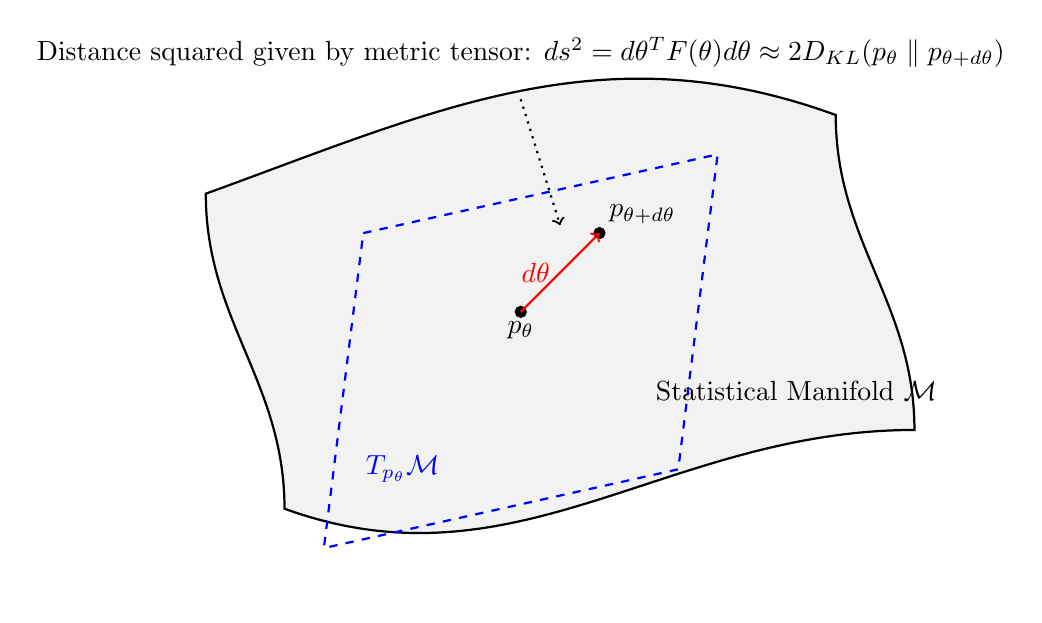
\begin{tikzpicture}
    % Manifold surface
    \draw[thick, fill=gray!10] (0,0) to[out=20,in=160] (8,1) to[out=270,in=90] (9,-3) to[out=180,in=340] (1,-4) to[out=90,in=270] cycle;
    \node at (7.5, -2.5) {Statistical Manifold $\mathcal{M}$};
    
    % Points
    \filldraw (4,-1.5) circle (2pt) node[below] {$p_\theta$};
    \filldraw (5,-0.5) circle (2pt) node[above right] {$p_{\theta+d\theta}$};
    
    % Tangent plane
    \draw[thick, blue, dashed] (2,-0.5) -- (6.5, 0.5) -- (6, -3.5) -- (1.5, -4.5) -- cycle;
    \node[blue] at (2.5, -3.5) {$T_{p_\theta}\mathcal{M}$};
    
    % Vector
    \draw[->, thick, red] (4,-1.5) -- (5,-0.5) node[midway, left] {$d\theta$};
    
    % Annotations
    \node[align=center] at (4, 1.8) {Distance squared given by metric tensor:   $ds^2 = d\theta^T F(\theta) d\theta \approx 2 D_{\text{KL}}(p_\theta \parallel p_{\theta+d\theta})$};
    \draw[->, dotted, thick] (4, 1.2) -- (4.5, -0.4);
\end{tikzpicture}
\caption{The statistical manifold $\mathcal{M}$ where each point is a distribution $p_\theta$. The tangent space $T_{p_\theta}\mathcal{M}$ is equipped with an inner product defined by the Fisher Information Matrix $F(\theta)$. The infinitesimal distance $ds^2$ between two distributions exactly corresponds to twice their KL divergence.}
\label{fig:fisher_manifold}
\end{figure}

\section{Numerical Example: The Univariate Gaussian}

To concretize these ideas, we explicitly compute the Fisher Information Matrix for a univariate Gaussian distribution. Let $p(x|\theta) = \mathcal{N}(x | \mu, \sigma^2)$, with parameter vector $\theta = [\mu, \sigma^2]^T$.

The log-likelihood of a single observation is:
\begin{equation*}
    \log p(x|\mu, \sigma^2) = -\frac{1}{2}\log(2\pi) - \frac{1}{2}\log(\sigma^2) - \frac{(x-\mu)^2}{2\sigma^2}
\end{equation*}

We first compute the score function (the first derivatives):
\begin{align*}
    \frac{\partial}{\partial \mu} \log p &= \frac{x-\mu}{\sigma^2} \\
    \frac{\partial}{\partial \sigma^2} \log p &= -\frac{1}{2\sigma^2} + \frac{(x-\mu)^2}{2(\sigma^2)^2}
\end{align*}

Next, we compute the second derivatives (the Hessian matrix entries):
\begin{align*}
    \frac{\partial^2}{\partial \mu^2} \log p &= -\frac{1}{\sigma^2} \\
    \frac{\partial^2}{\partial (\sigma^2)^2} \log p &= \frac{1}{2\sigma^4} - \frac{(x-\mu)^2}{\sigma^6} \\
    \frac{\partial^2}{\partial \mu \partial \sigma^2} \log p &= -\frac{x-\mu}{\sigma^4}
\end{align*}

Using Theorem~\ref{thm:fim_hessian}, we negate these and take expectations over $x \sim \mathcal{N}(\mu, \sigma^2)$. Recall that $\mathbb{E}[x-\mu] = 0$ and $\mathbb{E}[(x-\mu)^2] = \sigma^2$.
\begin{align*}
    F_{11} &= -\mathbb{E}\left[ -\frac{1}{\sigma^2} \right] = \frac{1}{\sigma^2} \\
    F_{22} &= -\mathbb{E}\left[ \frac{1}{2\sigma^4} - \frac{(x-\mu)^2}{\sigma^6} \right] = -\left( \frac{1}{2\sigma^4} - \frac{\sigma^2}{\sigma^6} \right) = \frac{1}{2\sigma^4} \\
    F_{12} &= F_{21} = -\mathbb{E}\left[ -\frac{x-\mu}{\sigma^4} \right] = 0
\end{align*}

Thus, the Fisher Information Matrix for the univariate Gaussian is diagonal:
\begin{equation}
    F(\mu, \sigma^2) = \begin{bmatrix}
        \frac{1}{\sigma^2} & 0 \\
        0 & \frac{1}{2\sigma^4}
    \end{bmatrix}
\end{equation}
This reveals that $\mu$ and $\sigma^2$ are orthogonal parameters under the Fisher metric. Notice how the information regarding $\mu$ diverges as variance approaches zero, perfectly echoing the intuition that smaller variance leads to higher precision in estimating the mean. The geometry of this space, defined by this metric, forms a hyperbolic geometry known as the Poincaré half-plane model.

\begin{horizon}
It is conjectured that the macroscopic generalization capabilities of large language models and other overparameterized networks are governed by the extreme degeneracy of the Empirical Fisher Information Matrix. In modern deep learning regimes, the FIM exhibits a tiny handful of massive eigenvalues and a vast, high-dimensional sea of near-zero eigenvalues. 

An open question is whether these degenerate ``flat directions'' explicitly guide stochastic gradient descent toward representations that generalize flawlessly, or if they merely reflect the massive functional redundancy of the network architectures. Furthermore, it is conjectured that regularizing optimization trajectories directly in the natural geometry of the statistical manifold---by navigating strictly along the near-zero eigen-directions of the FIM---could circumvent catastrophic forgetting and unlock lifelong learning at the theoretical limits of sample efficiency. Future work might show that the implicit regularization of SGD acts primarily as a mechanism for finding the lowest-rank subspace of the Fisher Information Matrix.
\end{horizon}

\section{Summary}

\begin{itemize}
    \item The \textbf{score function} $s(\theta; x) = \nabla_\theta \log p(x|\theta)$ points in the direction of steepest log-likelihood ascent. Its expected value over the true distribution is exactly zero.
    \item The \textbf{Fisher Information Matrix (FIM)} is defined as the covariance of the score function.
    \item Due to derivative identities, the FIM elegantly simplifies to the negative expected Hessian of the log-likelihood: $F(\theta) = - \mathbb{E}[ \nabla_\theta^2 \log p(x|\theta) ]$.
    \item Geometrically, the FIM serves as the metric tensor of the statistical manifold. It provides a local quadratic approximation to the Kullback-Leibler divergence between infinitesimally close probability distributions.
    \item A high-magnitude FIM corresponds to a sharply peaked log-likelihood landscape, where parameters are highly sensitive to data and easily identifiable. A low-magnitude FIM corresponds to flat regions of the loss landscape.
\end{itemize}

\section{Exercises}

\begin{enumerate}
    \item \textbf{Fisher Information of the Bernoulli Distribution:} Let $X \sim \text{Bernoulli}(p)$ for $p \in (0,1)$. Derive the (scalar) Fisher Information $F(p)$ using both the variance of the score function and the negative expected Hessian.
    \item \textbf{Reparameterization Invariance:} Let $\phi = h(\theta)$ be an invertible transformation of the parameter vector $\theta$. Using the chain rule, prove that the Fisher Information Matrix transforms according to the Jacobian of $h$: $F(\theta) = J^T F(\phi) J$, where $J = \frac{\partial \phi}{\partial \theta}$.
    \item \textbf{FIM of Linear Regression:} Consider a linear model $y = w^T x + \epsilon$, where $\epsilon \sim \mathcal{N}(0, \sigma^2)$ and $w \in \mathbb{R}^d$ is the parameter vector. The covariates $x$ are drawn from a distribution $P(x)$ with covariance matrix $\Sigma_x$. Show that the Fisher Information Matrix with respect to $w$ is exactly $\frac{1}{\sigma^2} \Sigma_x$. Explain how this connects the Fisher Information to the curvature of the Mean Squared Error (MSE) loss surface.
\end{enumerate}

% TODO-CITE: Ensure all named results are cited.
